\documentclass{article}
\usepackage{graphicx}
\usepackage{amsmath}
\usepackage{hyperref}
\usepackage{float}
\usepackage{subcaption} % for subfigures

\title{CSC311 Project Final Report}
\author{Group Members: \\ Zixuan Zeng 1008533419 \\ \\ }

\begin{document}

\maketitle

\section*{Part A}

\section*{Q1}

\subsection*{1.(a)}

\begin{figure}[H]
    \centering
    \begin{subfigure}{0.45\textwidth}
        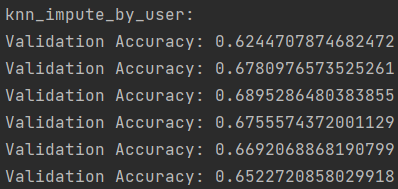
\includegraphics[width=\textwidth]{knn_impute_by_user_result.png}
    \end{subfigure}
    \hfill
    \begin{subfigure}{0.35\textwidth}
        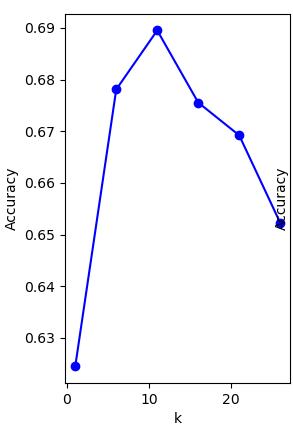
\includegraphics[width=\textwidth]{knn_impute_by_user_plot.png}
    \end{subfigure}
    \caption{Accuracy vs k for KNN Impute by User}
\end{figure}

\subsection*{1.(b)}

\begin{figure}[H]
    \centering
    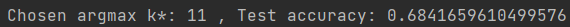
\includegraphics[width=\textwidth]{knn_impute_by_user_test.png}
    \caption{Test accuracy with k*}
\end{figure}

\subsection*{1.(c)}

The underlying assumption is that if question A is answered similarly by many students as question B, A’s predicted response from specific students matches that of question B.

\begin{figure}[H]
    \centering
    \begin{subfigure}{0.45\textwidth}
        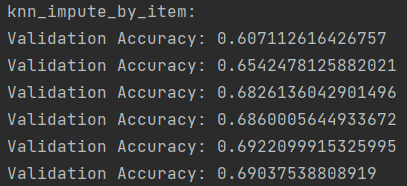
\includegraphics[width=\textwidth]{knn_impute_by_item_result.png}
    \end{subfigure}
    \hfill
    \begin{subfigure}{0.35\textwidth}
        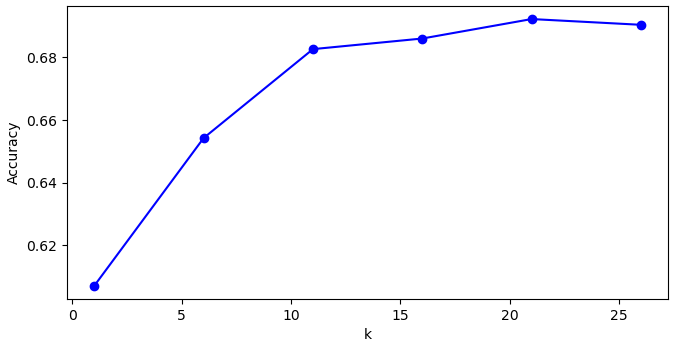
\includegraphics[width=\textwidth]{knn_impute_by_item_plot.png}
    \end{subfigure}
    \caption{Accuracy vs k for KNN Impute by Item}
\end{figure}

\begin{figure}[H]
    \centering
    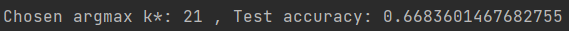
\includegraphics[width=\textwidth]{knn_impute_by_item_test.png}
    \caption{Test Accuracy with k*}
\end{figure}

\subsection*{1.(d)}
The test accuracy for the user-based method (0.6842) is higher than that for the item-based method (0.6684). Therefore, the user-based collaborative filtering method performs better than the item-based collaborative filtering method in this case.

\subsection*{1.(e)}
\begin{itemize}
    \item Computationally expensive. KNN practically has no training process. With large datasets, as the number of students/questions grow, the time required to compute the distances and to identify the nearest neighbors at test time grows significantly.
    \item Curse of Dimensionality. When the sparse\_matrix has too many missing values, it’s hard to find good nearest neighbors, since most points will be about the same distances. This affects the prediction accuracy.
\end{itemize}


\newpage
\section*{Q2}

\subsection*{2.(a)}

\[
p(c_{ij} = 1 | \theta_i, \beta_j) = \frac{\exp(\theta_i - \beta_j)}{1 + \exp(\theta_i - \beta_j)} = \sigma(\theta_i - \beta_j)
\]
log-likelihood:
\[
\log p(C | \theta, \beta) = \sum_{i}\sum_{j} \left[ c_{ij} (\theta_i - \beta_j) - \log (1 + \exp(\theta_i - \beta_j)) \right]
\]
The derivative of the log-likelihood with respect to $\theta_i$:
\[
\frac{\partial \log p(C | \theta, \beta)}{\partial \theta_i} = \sum_{j} \left[ c_{ij} - \sigma(\theta_i - \beta_j) \right]
\]
The derivative of the log-likelihood with respect to $\beta_j$:
\[
\frac{\partial \log p(C | \theta, \beta)}{\partial \beta_j} = \sum_{i} \left[ - c_{ij} + \sigma(\theta_i - \beta_j) \right]
\]

\subsection*{2.(b)}

\begin{figure}[H]
    \centering
    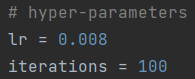
\includegraphics[width=0.3\textwidth]{2(b)1.png}
    \caption{Hyper-Parameters}
\end{figure}
\begin{figure}[H]
    \centering
    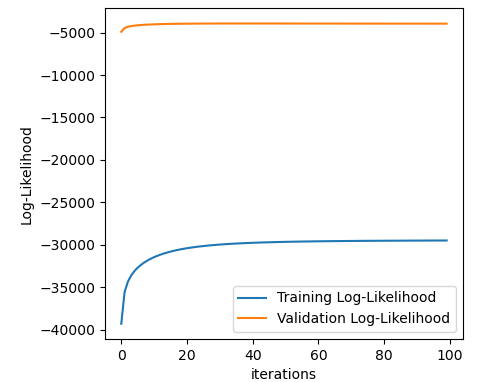
\includegraphics[width=0.5\textwidth]{2(b)2.png}
    \caption{Training and Validation Log-Likelihoods vs Iteration}
\end{figure}

\subsection*{2.(c)}
\begin{figure}[H]
    \centering
    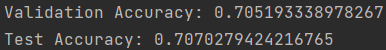
\includegraphics[width=0.6\textwidth]{2(c).png}
    \caption{Final Validation \& Test Accuracy}
\end{figure}

\subsection*{2.(d)}
The three curves are all in S shape, as the sigmoid function. They represent the probability of correct responses as a function of student ability $\theta$.\newline
It shows that students with a high ability have a high probability of answering correctly.\newline
Also, question with a high difficulty is skewed to the right, meaning it has a lower probability being answered correctly.
\begin{figure}[H]
    \centering
    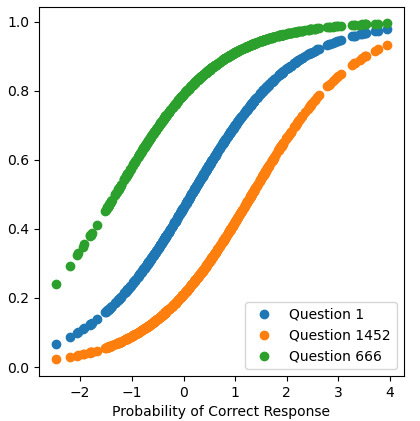
\includegraphics[width=0.6\textwidth]{2(d).png}
    \caption{Probability of Correct Response vs Theta}
\end{figure}


\newpage
\section*{Q3}


\newpage
\section*{Part B}

\end{document}
